% THE AMAZING BAXTER FEEDING ROBOT 
\documentclass[11pt]{report} %Letter size, letter type and report article structure

\usepackage{geometry}
\geometry{
 a4paper,
 total={210mm,297mm},
 left=40mm,
 right=20mm,
 top=40mm,
 bottom=30mm,
 }
 
\usepackage[spanish, english]{babel} % Recognize Spanish language

\usepackage[utf8]{inputenc} % Recognize Latin characters

\usepackage{amsmath} % Insert math formulas/functions

\usepackage{amsfonts} % Extended set of fonts

\usepackage{graphicx} % Include graphics in document

\usepackage{siunitx} % Consistent set of units with rules on how they are to be used

\usepackage{caption} % Caption for images, formulas and tables
\DeclareCaptionType{equ}[][] % Add caption functionalities to equations

\usepackage{natbib} % Cite library (to reference in APA format)
\usepackage[breaklinks=true]{hyperref} % Handle cross-referencing commands
\urlstyle{same}
\usepackage{url}

\usepackage{dirtytalk} % Add "in quotes" for specific parts of text (add "something")

\usepackage{comment} % Extra big-comments functionalities

\usepackage{textcomp} % For "R" and "TM" symbols

\usepackage{subcaption} % For sub-figures

\usepackage{array} % Usage of arrays

\usepackage{booktabs} % Better quality tables

\usepackage{longtable} % Allow tables to flow over page boundaries

\usepackage{makecell} % Extra functionalities to table cells tabs

\usepackage{multirow} % Extra functionalities to table cells row/cols

\usepackage{float} % Improve figures/tables position in page

\usepackage{algorithm} % Write algorithms easily

\usepackage[noend]{algpseudocode} % Improve pseudo-code algorithms

\usepackage[dvipsnames,table,xcdraw]{xcolor} % Color things

% Commands to generate list of equations
\usepackage{tocloft} % Package to generate list of equations
\newcommand{\listequationsname}{}
\newlistof{myequations}{equ}{\listequationsname}
\newcommand{\myequations}[1]{%
\addcontentsline{equ}{myequations}{\protect\numberline{\theequation}#1}\par}
\setlength{\cftmyequationsnumwidth}{2.5em}% Width of equation number in List of Equations


% These commands help us generate the "subsubsubseciton{}" title
\newcommand{\subsubsubsection}[1]{\paragraph{#1}\mbox{}\\}
\setcounter{secnumdepth}{4}
\setcounter{tocdepth}{4}


% Extra functionalities for vertical text
\newcommand*\rot{\rotatebox{90}}
\newcommand*\OK{\ding{51}}

% Reestablish specific low-level configurations
\renewcommand\theadalign{cb}
\renewcommand\theadfont{\bfseries}
\renewcommand\theadgape{\Gape[4pt]}
\renewcommand\cellgape{\Gape[4pt]}

% Remove first-indent in all document
\setlength\parindent{0pt}

% Avoid annoying "under full hbox oversize comment"
\hbadness = 2147483647
\vbadness = 2147483647

% Extra math operators values
\DeclareMathOperator{\T}{T}
\DeclareMathOperator{\g}{g}
\DeclareMathOperator{\f}{f}
\DeclareMathOperator{\F}{F}
\DeclareMathOperator{\h}{p}
\DeclareMathOperator{\p}{p}
\DeclareMathOperator{\U}{U}


% ---------------------------------------------------------

\begin{document}

% ---------------------------------------------------------

\begin{titlepage}

\begin{center}

\begin{Large}

\vspace*{1cm}
\textbf{ASSISTED ROBOTICS FOR FEEDING INDIVIDUALS WITH UPPER LIMB DISABILITIES}\\[6.5cm]

\textbf{Santiago García Arango} \\
\textbf{Elkin Javier Guerra Galeano}

\end{Large}

\vfill


\includegraphics[width=6cm]{assets/imgs/logoeia.png}\\

\begin{large}
\textbf{EIA UNIVERSITY}\\
\textbf{MECHATRONICS ENGINEERING}\\
\textbf{ENVIGADO, COLOMBIA}\\
\textbf{2021}\\
\end{large}
\end{center}
\end{titlepage}

% ---------------------------------------------------------

\begin{titlepage}
\begin{center}

\begin{Large}

\vspace*{1cm}
\textbf{ASSISTED ROBOTICS FOR FEEDING INDIVIDUALS WITH UPPER LIMB DISABILITIES}\\[3.5cm]

\textbf{Santiago García Arango}\\
\textbf{Elkin Javier Guerra Galeano}\\[2cm]

\end{Large}

\begin{large}

\textbf{Bachelor's final project to obtain the degree of:}\\
\textbf{Mechatronics Engineer}\\[2cm]

\textbf{Director of the project:}\\
\textbf{Dolly Tatiana Manrique Espíndola, M.Sc., Ph.D.}\\[1cm]

\end{large}

\vfill


\includegraphics[width=5cm]{assets/imgs/logoeia.png}\\

\begin{large}
\textbf{EIA UNIVERSITY}\\
\textbf{MECHATRONICS ENGINEERING}\\
\textbf{ENVIGADO, COLOMBIA}\\
\textbf{2021}\\
\end{large}

\end{center}
\end{titlepage}

% ---------------------------------------------------------

\begin{titlepage}
\begin{center}

\begin{Large}

\vspace*{1cm}
\textbf{ACKNOWLEDGMENTS}\\[3.5cm]

\textbf{Acknowledgments 1}\\

\end{Large}

\begin{Large}

\vspace*{3cm}

\textbf{Acknowledgments 2}\\

\end{Large}

\vfill

\end{center}
\end{titlepage}

% ---------------------------------------------------------

\pagenumbering{arabic} 

\tableofcontents



% ---------------------------------------------------------

\cleardoublepage
\listoffigures

% ---------------------------------------------------------

\cleardoublepage
\listoftables

% ---------------------------------------------------------

\cleardoublepage
\chapter*{List of Symbols}

\begin{longtable}{p{5mm} c p{120mm} }

\multicolumn{3}{l}{\textbf{Position Variables}}\\
\\
$\zeta$ & --- & Vector of something...\\
\\
\multicolumn{3}{l}{\textbf{Robot's parameters}}\\
\\
$P$ & --- & Centroid of ...\\

\\
\multicolumn{3}{l}{\textbf{Control Theory parameters}}\\
\\
$t$ & --- & Time ...\\

\\
\multicolumn{3}{l}{\textbf{Probability functions}}\\
\\
$\g(.)$ & --- & Probability function for ...\\

\\


\end{longtable}

% ---------------------------------------------------------

\cleardoublepage
\chapter*{List of Equations}

\listofmyequations

% ---------------------------------------------------------

\chapter*{Abstract}


The exponential growth of technology has made it possible to achieve new solutions to improve the human beings' quality of life. One of the areas that has experienced the greatest development in the last 20 years is robotics and its derivatives. Currently, there has been a significant increase in the number of people with motor disabilities in the upper limbs, including more than 10 million people with Parkinson's disease and several individuals who, due to other circumstances, have lost the mobility of their upper limbs. This group of people not only have major difficulties in the daily task of feeding, but can also experience severe problems of malnutrition and loss of self-esteem. This is why, in this project, an exploratory research will be conducted focused on the development of an active robotic solution, using Baxter Robot, which can give support in the feeding process for these individuals and, at the same time, has conditions of improvement compared to the robotic alternatives that exist in the current market.\\

This development will seek a positive impact for all individuals who fit within the exposed problem and a design methodology will be carried out, oriented to the search for a scalable solution, with the ability to recognize the position of the mouth of individuals through Computer Vision algorithms and with the advantage of being Open Source. It is expected that, at the end of this research, relevant advances will be generated in the development of active robotic solutions for the assistance of this population and the scientific knowledge of robotics in Colombia and the world.\\


\textbf{Keywords:} Robotics, Computer Vision, Control Theory, Denavit Hartenberg, Algorithms, Software, Anomalies, Active Feeding, Autonomous System.

% ---------------------------------------------------------

\chapter*{Introduction}

The overall population that have upper limb special needs or suffer from motor disabilities are more likely to have problems of malnutrition, a reduction in the performance in the activities of daily living, and loss of self-esteem  \citep{cite_ICBF_technical_article, cite_upper_limb_disabilities_self_steem}.\\

In this research project, we will dive into the design of a possible solution for these problems, using Baxter Robot as an active feeding solution that enables individuals to accomplish of the most important daily life activities: eating.\\

The project's scope covers some important stages for the complete design: \\

\begin{enumerate}
    \item General understanding of the overall design based on human-being needs.
    \item Specific planning and implementation of each sub-system of the complete design.
    \item Practical experiments to validate the functionalities of the designs.
    \item Final results analysis and next steps for future improvements.
\end{enumerate}

Throughout this article, we will be exposing the theoretical and practical steps that were involved in the design of the Baxter Feeding Robot solution.\\

At the end of the article, we will expose the most important ethical and real life considerations of designing a robotics solution that interacts with human beings.

% ---------------------------------------------------------

\chapter{Initial Steps}

\section{Understanding the problem}

\subsection{Problem's context and analysis}

According to the Technical Guide of the Food and Nutrition Component for the Population with Disabilities of the Colombian Institute of Family Welfare (ICBF), this group of individuals are more likely to have nutritional problems \citep{cite_ICBF_technical_article}. Likewise, individuals with upper limb disabilities, have a significant reduction in activities of daily living (especially feeding) and may become impaired in their psychological state \citep{cite_upper_limb_disabilities_self_steem}.\\

It is estimated that there are more than 10 million people with Parkinson worldwide, of which a significant percentage have critical mobility problems in their upper extremities \citep{cite_parkinson_foundation_total_cases}. The incidence of people with Parkinson's disability increases with the age of the individuals, but there is an approximate 4\% of them who are diagnosed before the age of 50 years. According to studies conducted by the Parkinson Foundation (PF), men are more likely than women to have this disease. Another factor that is of relevance to this problem is that there is currently a higher prevalence of pain and disabilities in upper limbs in young university populations, which implies an increase in the group of people who will have joint disabilities in the future and will be more likely to present malnutrition problems due to the difficulties of performing the task of feeding by their own hands \citep{cite_park_active_robot_assisted_feeding}.\\

This is why it is necessary to look for technological solutions that allow this group of individuals to receive support and assistance in daily tasks, especially feeding. Considering this context, a branch of robotics known as \say{Assisted Robotics} is of interest, where robotic systems seek to support individuals with disabilities to perform daily tasks \citep{cite_assited_robotics_stanford_lecture_jaffe}.\\

Advances in assisted robotics have led to the development of various systems that seek to assist people with disabilities in the task of feeding (scooping). There are commercial robotic platforms, which seek to fulfill the need to feed patients with upper limb motor disabilities, but these have a number of limitations that restrict and limit their ideal performance. The best known commercial robotic systems for these tasks, such as Myspoon, Bestic Arm, Meal Buddy, Mealtime and Obi, are passive in nature. This means that they do not have the ability to adapt to the dynamic conditions of the user's mouth position, nor the ability to detect anomalies in the feeding process \citep{cite_park_active_robot_assisted_feeding}.\\

A restriction of great relevance found in commercial robotic systems is that they are not able to adapt their behavior to temporary changes in the position of the user's mouth, because their system is passive, limiting the ability to know this information that is required for a correct feeding action. Another limitation of these systems is that they fail to identify anomalies or strange behaviors in the feeding process, generating additional risks for the patient in case of any emergency or eventuality. Finally, these systems are implemented with restricted code, limiting their modifications in the source code and restricting the possibility of replicating these algorithms for the entire population that may need them.\\

Taking into account this worldwide problem, with the aim of improving the quality of life for individuals who have motor disability problems in upper limbs, it is important and of great relevance to seek an active robotic solution that can support the feeding process of these individuals, with a number of significant improvements over current commercial robotic systems. This solution should be able to adapt its dynamic movements constantly according to the position of the user's mouth, be aware of the environment, check for possible anomalies that may occur in it, be accessible and affordable for the population affected by their motor disabilities, be scalable to any other similar robotic system that is programmable and, similarly, should promote and seek innovation and the technological development of related robotic systems in Colombia and the world.\\

Based on the previous arguments, this research will aim to solve the question of:
How to implement an active robotic system for feeding (scooping) patients with motor disabilities in upper extremities, using the Baxter cobot of the EIA University?\\

In order to find a solution for the lack of active commercial robotic systems for feeding individuals, that also have the ability to adapt their movements according to the position of the user's mouth and the conditions of the environment, based on Mechatronics Engineering, several technological solutions can be proposed to integrate the main branches of electronics, mechanics, control systems and software development, to find an optimal solution to this identified problem \citep{cite_university_eia_general}.\\

This is why it is being proposed to develop a programmed robotic solution, which has an user interface activated by voice commands or friendly buttons, to generate a reliable and safe solution for the needs of people with motor disabilities in the upper limbs, to perform the daily activity of feeding. This solution, being open source, can be easily extrapolated to any programmable robotic platform, generating an additional step in the development of assisted robotic systems.\\

Considering the concept of assisted robotics and the importance of helping these individuals, the answer to provide a viable, scalable and safe solution to this problem is the usage of collaborative robots under the approach of working with humans  \citep{cite_rethink_robotics_baxter_factory_worker}. This can be achieved through various robotic alternatives, but it was decided to use Baxter robot from the company Rethink Robotics, which was developed under the concept of \say{cobot}, that means, a collaborative robot to work together with humans and is available in the laboratories of the university campus \citep{cite_university_eia_general}.\\

Due to the arguments exposed above, we want to look for a solution with the Baxter cobot, using the internal architecture of the software components integrated with the infrastructure offered by this company. This solution must be able to integrate the development of the software architecture, computational algorithms, kinematic models, video processing with computer vision, user interface,  and the necessary connections of these components for the correct implementation of the robotic solution, which will be focused on improving the quality of life of individuals who will benefit from this technology. Likewise, the system will represent a series of elements scalable to any other robotic platform with similar operating conditions and will seek to generate a positive impact on the development of assisted robotic systems for the community.\\

The development of a solution to this problem has multiple benefits, both for individuals with motor disabilities in the upper limbs, as well as for the scientific and medical community in Colombia. That is why, by developing this project, we want to take an additional step in the research and applications of assisted robotics, in order to seek to improve the quality of life of people with motor disabilities in the upper limbs.\\

This contribution can allow a person with these conditions, to perform the essential activity of feeding, without the need of having an external person performing this task. In the same way, this generates an increase in self-esteem and quality of life for these individuals.
At the same time, a key factor of the project is that it will positively contribute to the pursuit of three of the global objectives of sustainable development, especially: \say{Health and well-being}, \say{Industry, innovation and infrastructure} and \say{Reduction of inequalities} \citep{cite_united_nations_sustainable_development}.\\

In addition to the previous reasons, one of the most important motives for carrying out this project is that there is a large gap between the robotics of the leading countries in technology and Colombian robotics. This is why the project will provide a methodological approach for robotics research and a technological progress that can be replicated in any Colombian institution that has access to robotic platforms, generating a community that aims to improve robotic developments at a national level.\\


% ---------------------------------------------------------

\newpage

\section{Research objectives}

In this chapter, we will dive into the objectives of the research that are expected by the end of the project.\\

It is of high importance to have a general and specific planning of the objectives to be developed in the evolution of the project. The following are the proposed objectives for the final scope of the solution proposed in this degree project.\\

\subsection{General objective}

Implement an active feeding system (scooping) for patients with motor disabilities in upper extremities, using the Baxter cobot of EIA University.

\subsection{Specific objectives}

\begin{enumerate}

\item Generate the smooth paths and trajectories between the position of the tool and the user's mouth, through a face detection system, which returns the absolute coordinates of the user's mouth based on the OpenCV library.

\item Implement a control strategy for tracking the proposed paths and trajectories, through a kinematic processing, to generate the action commands to move the joints of the Baxter cobot and validate its performance with a control algorithm, using the current position of the user's mouth as direct feedback to the system.

\item Design an algorithm for anomaly or error detection in the feeding process, which provides an action signal to stop the system in case of unexpected events.

\item Integrate the sub-systems of path and trajectory generation, control strategy and anomaly detection, using the Robot Operating System (ROS) libraries and tools.

\item Develop an user interface, which enables to send the commands to start the feeding and, if necessary, to stop the process.

\end{enumerate}

% ---------------------------------------------------------

\newpage

\section{Reference framework}

\subsection{Historical background}

Robotics was initially conceived as one of the branches of science with the greatest impact on industrial automation and processes that allow repetitive tasks to be performed. However, the concept of robotics has been expanding its scope and applications, because there are new sectors and scenarios where robots with new objectives and capabilities are becoming more frequent. Some of these scenarios are focused on improving the quality of life of human beings. Two major current scenarios of robotics are: assisted robotics and collaborative robotics \citep{cite_service_robotics_and_human_labor}.\\

Assisted robotics refers to all types of robots that have the ability to collect information from the environment, process that information, and perform tasks or actions that benefit individuals with any type of disability \citep{cite_assited_robotics_stanford_lecture_jaffe}. Based on this definition, it can be concluded that assisted robotics enables the improvement of the quality of life of people with any disability, including the human beings with motor impairments in the upper limbs.\\

The existing studies and researches related to robotics focused on patient feeding have had great advances in the last 10 years. Furthermore , it can be visualized that most current works are directed to the search and improvement of systems for feeding individuals in an active way, i.e., systems that autonomously feed patients \citep{cite_park_active_robot_assisted_feeding}.\\

In order to effectively structure and summarize some of the researches, degree papers and patents related to the topic of assisted robotics, a literature review of the last few years was carried out to collect the objectives, methodologies, solutions, strategies and conclusions of these projects. Some of the most relevant ones are presented below:\\

In the article \say{Active robot-assisted feeding with a general-purpose mobile manipulator: Design, evaluation, and lessons learned} \citep{cite_park_active_robot_assisted_feeding}, published in the scientific journal \say{Robotics and Autonomous Systems 124}, an overview of robotic systems focused on patient feeding is presented, providing a contrast of commercial platforms and those under research and development. In this study, an algorithm and software architecture based on a PR2 robotic manipulator was implemented to achieve autonomous feeding of patients with upper extremity disabilities. The characteristics, methodologies and solutions found in similar projects were presented, making a contrast between them and exposing new proposals that made use of some of the knowledge found by all previous investigations. Besides, the article reflects an exhaustive work with a good overview of previous knowledge to develop similar robotic solutions in the future, as it not only exposes the development of their research in the particular context, but also proposes the most important elements to take into account in assisted robotics projects.\\

Another study of major relevance to the state of the art of assisted robotics is \say{SAM, an Assistive Robotic Device Dedicated to Helping Persons with Quadriplegia: Usability Study} \citep{cite_SAM_an_assisted_robotic_device_to_help_quadriplegia_persons}. In this research, important concepts about assisted robotics and the current delimitation of various robotic applications in this area of knowledge are exposed. Likewise, the authors expose the importance of defining the factors for the success of robotic tasks, since the evaluation of the viability of implementation, is linked to correctly defining the success of the corresponding subroutines. Likewise, several interfaces that can be implemented for quadriplegic users are shown and their advantages and disadvantages are contrasted.\\

Additionally, by researching related studies, a very important element was identified in the development of a robotic system that interacts with individuals: the detection of anomalies. To give context to this feature, two research articles were analyzed, which were \say{A Multimodal Execution Monitor with Anomaly Classification for Robot-Assisted Feeding} \citep{cite_multimodal_execution_monitor_with_anomaly_classification} and \say{A Multimodal Anomaly Detector for Robot-Assisted Feeding Using an LSTM-based Variational Autoencoder} \citep{cite_multimodal_anomaly_detector_for_robot_assisted_feeding_LSTM}. From these scientific papers, we gained a deeper insight into more than 5 mathematical methodologies for strategically detecting anomalies. Similarly, they expose analytical procedures that are of great importance in the structure of algorithms that focus on searching for anomaly patterns, enabling us to have these as a starting point to develop new strategies for future robotic implementations.\\

Regarding patents, the United States patent called \say{Mobile human-friendly assistive robot} \citep{cite_patent_mobile_human_friendly_assistive_robot} was mainly reviewed. In this publication, it was possible to identify a viable structure for the communications architecture developed in assisted robotics projects, enabling the selection of the principal and secondary components in the infrastructure to be developed for robotic projects.\\


A very interesting article for the understanding of assisted robotics projects is \say{Robots for humanity: Using collaborative robots to help people with disabilities} \citep{cite_robot_for_humanity_empower_people_with_disabilities}. In this document, it is exposed the relevance of simplifying the graphical user interface, through the use of mathematical tools such as elliptic coordinates and an interface compatible with sound commands. Similarly, the authors propose a strategic error detection system by translating the forces implemented by the robotic system in different mathematical approaches.\\


\subsection{Theoretical background}

Primarily, it is important to delimit the suggested solution within a specific context, explaining the use cases for the conditions of the technology applied and the people who will benefit from it. A first group of people who benefit are individuals who suffer from advanced Parkinson's disease and are unable to perform smooth feeding movements due to tremors, shaking or bradykinesia in their hands \citep{cite_parkinsons_disease_symptomps_mayo_clinic}. Likewise, there is a large number of people with motor disabilities in upper limbs that fail to be categorized into a specific group of individuals, but because of their age conditions, diseases, symptoms or accidents, they have significant difficulties in the daily process of feeding and can be highly benefited by the technological advances that this solution provides.\\

There are a number of preliminary concepts of critical importance for the understanding and development of the overall project. The most relevant concepts and simple contextualization of these by branches of study are presented below.\\

\subsubsection{Robotic concepts}

Robotics is a field of engineering that has significantly impacted the technological development of manufacture, industrial, medical, security, and human support industries, among others \citep{cite_robots_in_automotive_manufactoring_top_6_applications}. In order to have a solid foundation of the theoretical and mathematical foundations of robotic systems models, it is necessary to go into detail on some concepts and terminology related to the subject. Some of these concepts and terminologies will be discussed in more detail below.\\

\subsubsubsection{Transformation homogeneous matrices}

A transformation matrix is an important mathematical tool to generate expressions of linear systems that have a combination of translational and rotational motions in space.

Given the reference systems \{A\} and \{B\}, with unit vectors that meet the dextrorotating criteria of a linear system, a rotation matrix can be defined as a matrix representation that compacts the rotations that must be performed in space to bring the reference frame {A} to {B} by the three unit vectors expressing the directions of these spatial changes ${_B^A}\hat{X}$, ${_B^A}\hat{Y}$, ${_B^A}\hat{Z}$ \citep{cite_craig_robotics}.\\

To generate the resulting rotation matrix between systems \{A\} and \{B\}, we proceed to create a matrix with the following structure:

\begin{equ}[H]
\begin{equation} \label{eq:rotation_matrix_general_structure}
    _{B}^{A}\textrm{R} = 
    \begin{bmatrix}
    {_B^A}\hat{X} & {_B^A}\hat{Y} & {_B^A}\hat{Z}
    \end{bmatrix} =
    \begin{bmatrix}
    r_{11} & r_{12} & r_{13}\\ 
    r_{21} & r_{22} & r_{23}\\ 
    r_{31} & r_{32} & r_{33}
    \end{bmatrix}
\end{equation}
\myequations{Rotation matrix general structure}
\caption{Rotation matrix general structure}
\end{equ}

As show in equation \ref{eq:rotation_matrix_general_structure}, the rotation matrix structure is a 3 by 3 matrix with orthogonal conditions with determinant 1. These properties are useful to compute some important matrix multiplications for different types of linear problems.\\

The next relevant conceptual step for the creation of a homogeneous transformation matrix is the translation. To represent a translation from a coordinate system to a point P, at least one vector indicating the relative translations of each of the unit vectors governing the orthogonal basis is required $\hat{X}$, $\hat{Y}$, $\hat{Z}$ :

\begin{equ}[H]
\begin{equation} \label{eq:translation_vector_general_structure}
    _{}^{A}\textrm{P} = \begin{bmatrix}
    P_{x}\\ 
    P_{y}\\ 
    P_{z}
    \end{bmatrix}
\end{equation}
\myequations{Position translation vector structure}
\caption{Position translation vector structure}
\end{equ}

Finally, when a mathematical strategy is required to represent both the translation and rotation of a system in space, this transformation can be expressed as a transformation matrix with the following structure:

\begin{equ}[H]
\begin{equation} \label{eq:tranformation_matrix_general_structure}
    _{B}^{A}\textrm{T} = 
    \begin{bmatrix}
    _{B}^{A}\textrm{R} & _{}^{A}\textrm{P}\\ 
    \O  & 1
    \end{bmatrix} = 
    \begin{bmatrix}
    r_{11} & r_{12} & r_{13} & P_{x}\\ 
    r_{21} & r_{22} & r_{23} & P_{y}\\ 
    r_{31} & r_{32} & r_{33} & P_{z}\\ 
    0 & 0 & 0 & 1
    \end{bmatrix}
\end{equation}
\myequations{Transformation matrix general structure}
\caption{Transformation matrix general structure}
\end{equ}

\subsubsubsection{Forward Pose kinematics}

The Forward Pose Kinematics (FPK) transform are all those equations that relate the behavior of a robotic system, taking into account as input parameters the values of each of the joints associated with the degrees of freedom, allowing to obtain as output the absolute Cartesian coordinates for the robot's end effector \citep{cite_craig_robotics}.\\

There are two main techniques for obtaining the Forward Pose Kinematics (FPK) of a robotic system, the geometrical method and the analytical method. In the geometrical method, a set of equations obtained from the model of the robot in the Cartesian space is formulated and a series of expressions is sought to represent the absolute spatial coordinates of the global system, that is, the expected position of the end effector. For this method, it is common to refer to the desired point as \say{Ptool} \citep{cite_craig_robotics}.\\

The analytical approach is a systematic methodology where rigorous steps must be followed to obtain the transformation matrices that govern the robotic system. This approach is divided into three main stages, which are: locating the axes of rotation or translation of each degree of freedom (DOF), defining the origin and direction of rotation of the main axes of each degree of freedom and, finally, locating the missing axes to obtain a series of reference systems that fulfill the desired translations and rotations \citep{cite_barrientos_robotics_book}.\\

The following is an example of the FPK of a revolute-revolute planar robot:

\begin{center}
\includegraphics[width= 0.4\textwidth]{\string "assets/pdfs/reference_framework/RR_general_draw".pdf}
\bigbreak
\begin{minipage}{\linewidth} %Keep image/PDF in only 1 page
\captionof{figure}{General schematic model for RR planar robot.}\label{fig_general_rr_drawing.}
\end{minipage} \end{center}

By solving the FPK of the RR robot, from fig[\ref{fig_general_rr_drawing.}], it can be shown that the equations governing the position and orientation of the robot tool are the following:

\begin{equ}[H]
\begin{equation} \label{eq:results_rr_robot_fpk_example}
    \begin{split}
        P_{Tx} & = L_{1} \cdot cos(\theta_{1}) + L_{2} \cdot cos(\theta_{1} + \theta_{2}) \\
        P_{Ty} & = L_{1} \cdot sin(\theta_{1}) + L_{2} \cdot sin(\theta_{1} + \theta_{2}) \\
        \alpha & = \theta_{1} + \theta_{2}
    \end{split}
\end{equation}
\myequations{Forward Pose Kinematics results for RR robot example.}
\caption{Forward Pose Kinematics results for RR robot example.}
\end{equ}

\subsubsubsection{Inverse Pose Kinematics}

The Inverse Pose Kinematics (IPK), are all those equations that relate the behavior of a robotic system, having as input parameters the absolute Cartesian values, allowing finding the equivalent values of each one of the degrees of freedom (DOF) of a robotic system \citep{cite_craig_robotics}.

It is common for a robot to have different kinds of actuators for the linear and rotational movements of its joints, so it is of high importance to obtain a series of expressions that can describe the possible values of these joints, for a specific position of the robot's tool.\\

Based on the following schematic, we can find the IPK of the given RR robot example:

\begin{center}
\includegraphics[width= 0.4\textwidth]{\string "assets/pdfs/reference_framework/RR_angles_convention".pdf}
\bigbreak
\begin{minipage}{\linewidth} %Keep image/PDF in only 1 page
\captionof{figure}{General schematic with the angles convention for RR planar robot.}\label{fig_rr_angles_exmple_schematic}
\end{minipage} \end{center}


The equations that describe the IPK of a planar RR robot, as shown in Fig[\ref{fig_rr_angles_exmple_schematic}], are shown as follows:

\begin{equ}[H]
\begin{equation} \label{eq:results_rr_robot_ipk_example}
    \begin{split}
        L_{T} & = \sqrt{P_{Tx}^2 + P_{Ty}^2} \\
        \gamma & = atan2(P_{Tx}, P_{Ty}) \\
        \alpha & = acos \left( \frac{L_{T}^2 + L_{1}^2 - L_{2}^2}{2 \cdot L_{1} \cdot L_{T}} \right) \\
        \beta & = acos \left( \frac{L_{1}^2 + L_{2}^2 - L_{T}^2}{2 \cdot L_{1} \cdot L_{2}} \right) \\
        \theta_{1} & =  \gamma + \alpha \\
        \theta_{2} & = \beta - \pi
    \end{split}
\end{equation}
\myequations{Inverse Pose Kinematics results for RR robot example.}
\caption{Inverse Pose Kinematics results for RR robot example.}
\end{equ}

It's important to state that in robotic systems with more than one degree of freedom, it is possible to reach the same point in space through different configurations of its joints, usually known as \say{elbow up} and \say{elbow down} for the same joint. For this reason, it should be kept in mind that there could be more possible solutions, as more degrees of freedom are available.\\

\subsubsubsection{Path planning}

Path planning refers to the strategy of generating spatial routes to achieve the movements of a robotic system between two points in space, using techniques to find the most appropriate route, taking into account the constraints of the environment. The methods to generate the paths may vary according to the type of robot and the dynamic conditions that it has to face in the context of the surrounding environment. It is relevant to mention that, in order to generate the planning of a given path, a series of preliminary elements of the environment must be previously known through integrated sensors that are able to translate their signals into valuable information for the robot \citep{cite_wheeled_robots_autonomous_book}.\\

\subsubsubsection{Higher-order polynomials trajectories}

Soft trajectories are parametric vectors that define all the points in space that a robotic manipulator must follow, in order to change its position in space from an initial point to an final point, having as input the desired position, velocity and acceleration conditions. There are two mathematical trajectories that allow an acceptable robotic performance, these are the 3\textsuperscript{rd} and 5\textsuperscript{th} order trajectories. The 5\textsuperscript{th} order trajectories are those that allow the control of any kind of dynamic system, with a correct control of variables such as jerk \citep{cite_craig_robotics}.
In this section, it is important to understand in depth the mathematical expressions that govern a behavior with 3\textsuperscript{rd} and 5\textsuperscript{th} order trajectories.\\

The 3\textsuperscript{rd} order trajectories fulfill the following mathematical expressions:


\begin{equ}[H]
\begin{equation} \label{eq:equations_for_third_order_trajectories}
    \begin{split}
        \theta(t) &= a_{0} + a_{1} \cdot t + a_{2} \cdot t^2 + a_{3} \cdot t^3\\
        a_{0} &= \theta_{0}\\
        a_{1} &= \dot{\theta_{0}} \\
        a_{2} &= \frac{3(\theta_{f} - \theta_{0})}{t_{f}^2} - \frac{2 \dot{\theta_{0}}}{t_{f}} - \frac{\dot{\theta_{f}}}{t_{f}}\\
        a_{3} &= \frac{2(\theta_{0} - \theta_{f})}{t_{f}^3} + \frac{(\dot{\theta_{0}} + \dot{\theta_{f}})}{t_{f}^2}
    \end{split}
\end{equation}
\myequations{Equations for third order trajectories.}
\caption{Equations for third order trajectories.}
\end{equ}

Similarly, the 5\textsuperscript{th} order polynomial trajectories, follow these mathematical equations:


\begin{equ}[H]
\begin{equation} \label{eq:equations_for_fifth_order_trajectories}
    \begin{split}
        \theta(t) &= a_{0} + a_{1} \cdot t + a_{2} \cdot t^2 + a_{3} \cdot t^3 + a_{4} \cdot t^4 + a_{5} \cdot t^5\\
        a_{0} &= \theta_{0}\\
        a_{1} &= \dot{\theta_{0}} \\
        a_{2} &= \frac{\Ddot{\theta_{0}}}{2}\\
        a_{3} &= \frac{20\theta_{f} - 20\theta_{0} - (8\dot{\theta_{f}} + 12\dot{\theta_{0}})t_{f} - (3\ddot{\theta_{0}} - \ddot{\theta_{f}})t_{f}^2}{2t_{f}^3}\\
        a_{4} &= \frac{30\theta_{0} - 30\theta_{f} + (14\dot{\theta_{f}} + 16\dot{\theta_{0}})t_{f} + (3\ddot{\theta_{0}} - 2\ddot{\theta_{f}})t_{f}^2}{2t_{f}^4}\\
        a_{5} &= \frac{12\theta_{f} - 12\theta_{0} - (6\dot{\theta_{f}} + 6\dot{\theta_{0}})t_{f} - (\ddot{\theta_{0}} - \ddot{\theta_{f}})t_{f}^2}{2t_{f}^5}
    \end{split}
\end{equation}
\myequations{Equations for fifth order trajectories.}
\caption{Equations for fifth order trajectories.}
\end{equ}



\subsubsubsection{Assistive robotics}

A collaborative robot or \say{cobot} is a robotic device capable of manipulating objects in cooperation with or providing assistance to humans. Thus, cobots have the ability to perform critical tasks for humans or work in conjunction with them \citep{cite_robots_for_collaboration_with_human_operators}. A field of collaborative robotics is assisted robotics, defined as any robotic device that performs tasks for the benefit of people with disabilities in the context of activities of daily living \citep{cite_assited_robotics_stanford_lecture_jaffe}.\\

\subsubsubsection{Robot's workspace}

In the context of robotics, the workspace is defined as all possible spatial locations where a robotic manipulator is able to reach thanks to the strategic movement of its degrees of freedom independently. The mathematical delimitation of this is a process that requires finding multiple possible spatial solutions for the maximum access points and plotting them in a simulation environment. It is common for manufacturers of industrial robots to provide a detailed review and explanation of the workspace in the robot's data-sheets, because it varies not only by geometric constraints, but also by the mechanical restrictions existing in the joint connections \citep{cite_craig_robotics}.\\


\subsubsubsection{Baxter cobot}

Baxter is a collaborative robot developed for the industrial sector by the company Rethink Robotics. It was designed with a series of sensors, cameras and control systems that allows it to work in a cooperative environment and to adapt easily to its workspace \citep{cite_rethink_robotics_official_page}.\\

Baxter was announced to the community in September 2011 and can be broadly defined as a two-armed robot with 7 degrees of freedom in each arm. Baxter was introduced to the market as a robot specialized in simple collaborative tasks, such as loading and unloading, organizing and interacting with materials \citep{cite_sdk_baxter_rethink_robotics}. Likewise, being a robot that seeks to interact with humans, it has a screen that simulates the face of the Baxter cobot and additional safety protection features that will be considered in the development of the project.

\begin{figure}[H]
    \centering
    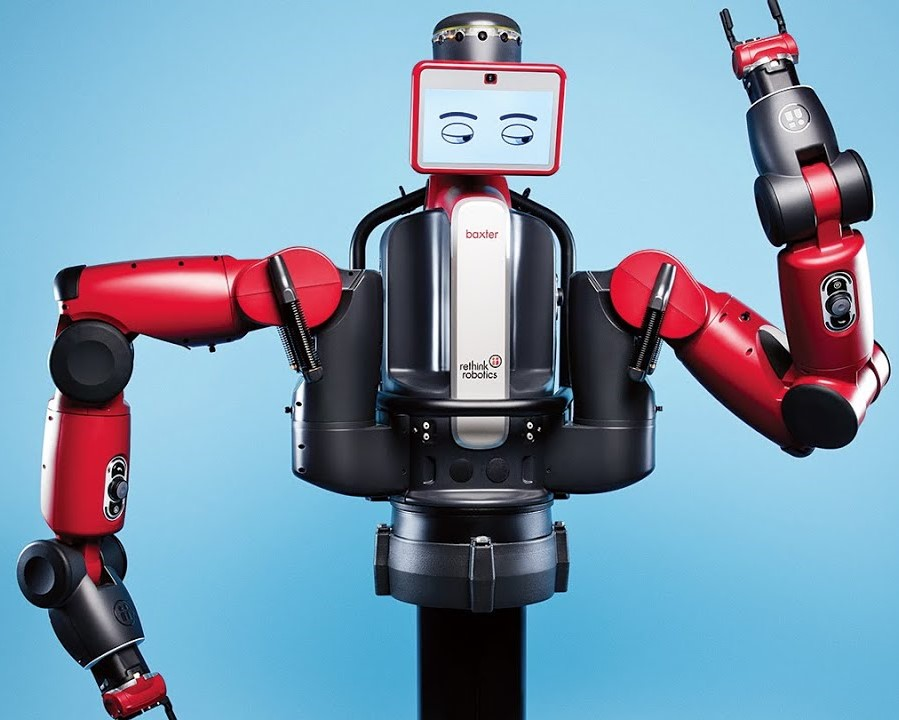
\includegraphics[width=0.75\linewidth]{assets/imgs/reference_framework/main_baxter.jpg}
    \caption{Front view for Baxter cobot. Taken from \citep{cite_youtube_baxter_robot_future_employee}.} 
    \label{fig_baxter_main_image}
\end{figure}

Considering the general specifications, it is of major relevance to have a clear understanding of each one of the degrees of freedom that the Baxter joints have and their standard nomenclatures for their operation. The following figure is an image of the official technical data-sheet of Baxter's documentation, where the seven DOF and their names are illustrated:

\begin{figure}[H]
    \centering
    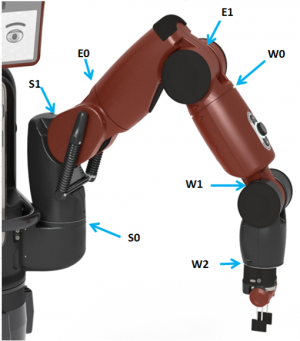
\includegraphics[width=0.4\linewidth]{assets/imgs/reference_framework/baxter_joint_names.png}
    \caption{Baxter left joint names for each DOF. Taken from \citep{cite_baxter_joint_names_from_sdk_wiki}.} 
    \label{fig_baxter_joint_names}
\end{figure}

When working and programming the Baxter cobot, it is essential to have a good understanding of the workspace conditions and the general restrictions of each of the degrees of freedom. The following image is a visual illustration of Baxter's workspace and its numerical limits for each joint:

\begin{figure}[H]
    \centering
    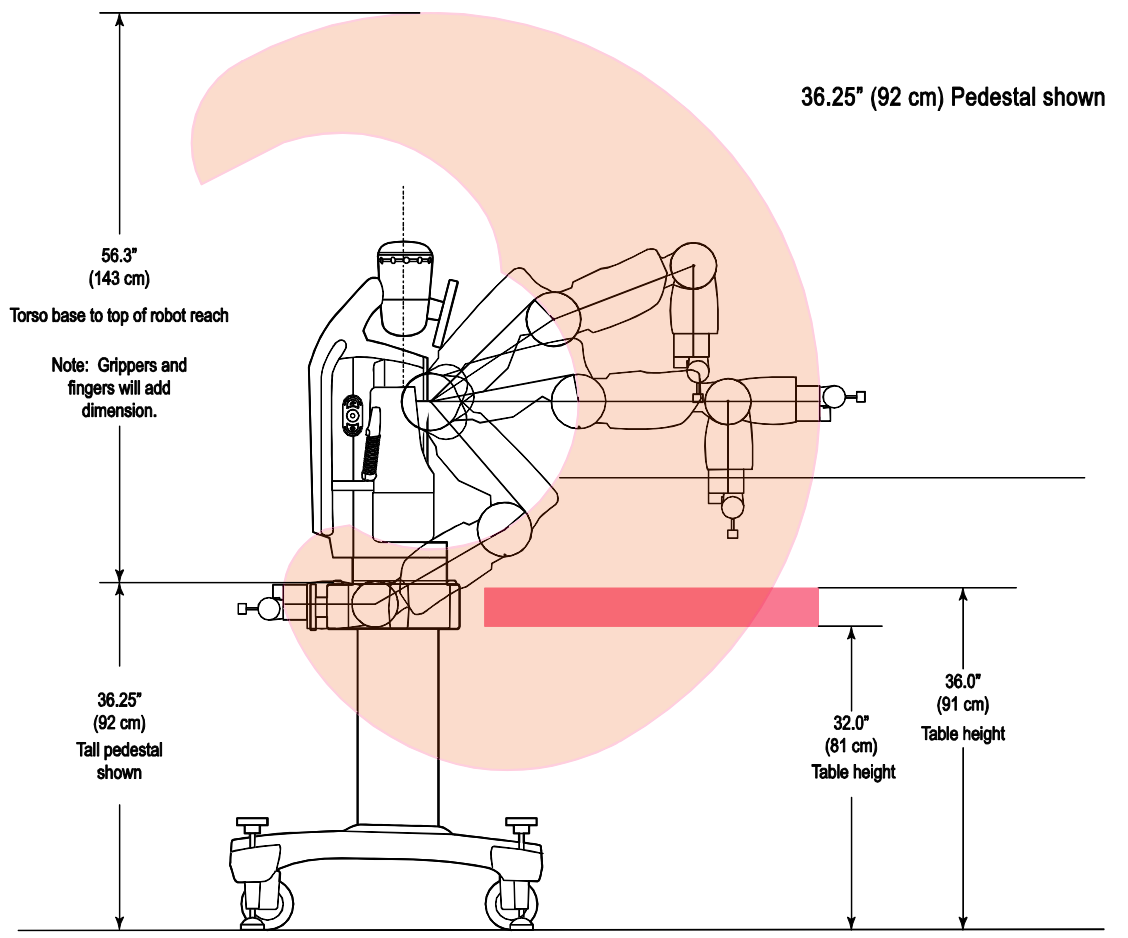
\includegraphics[width=0.65\linewidth]{assets/imgs/reference_framework/baxter_workspace_side_view.png}
    \caption{Baxter workspace side view. Taken from \citep{cite_baxter_workspace_from_sdk_wiki}.} 
    \label{fig_baxter_workspace_1}
\end{figure}

\begin{figure}[H]
    \centering
    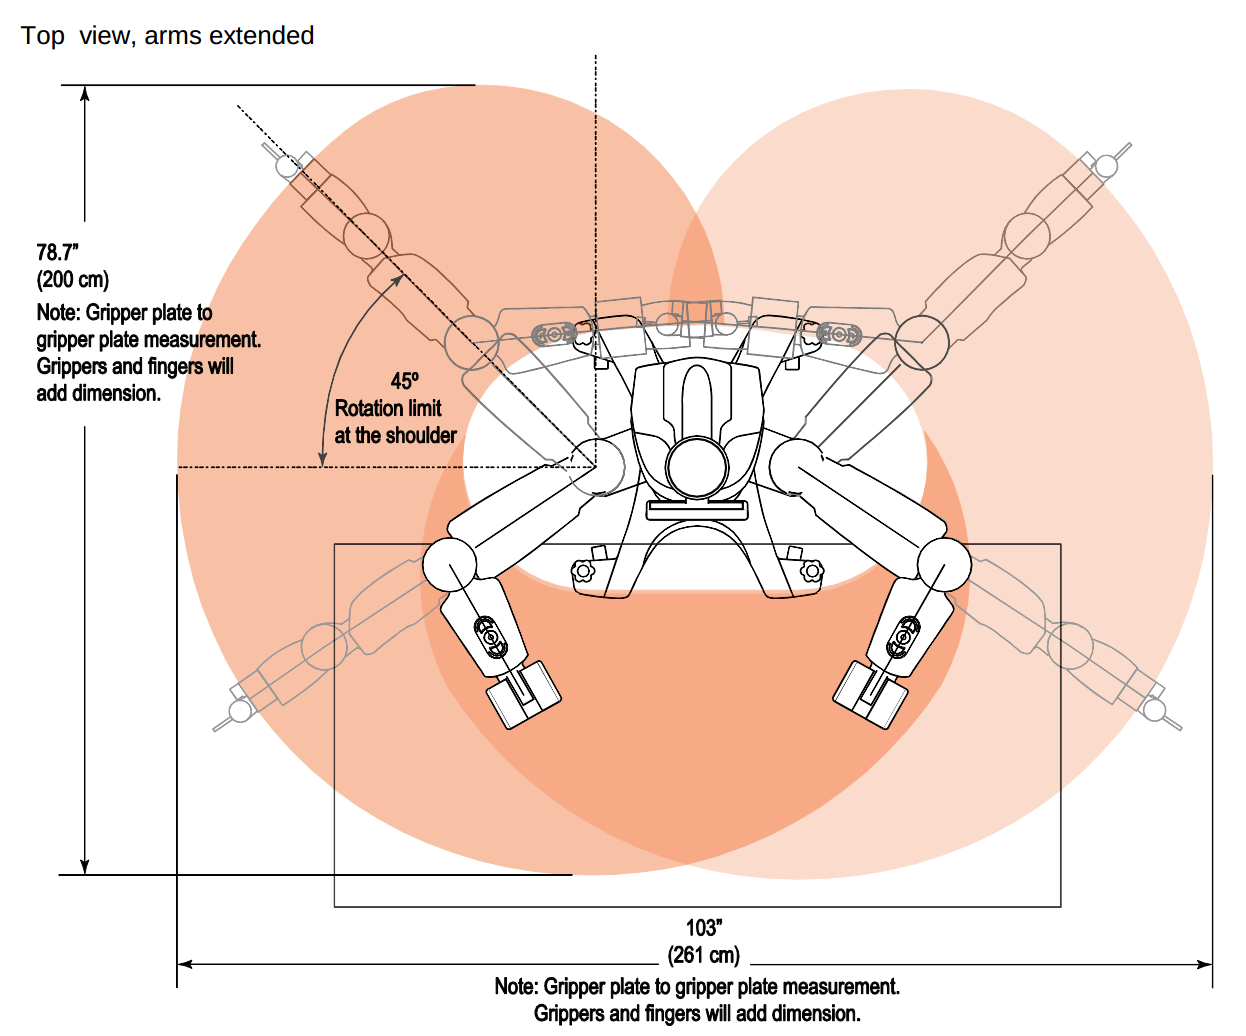
\includegraphics[width=0.65\linewidth]{assets/imgs/reference_framework/baxter_workspace_top_view.png}
    \caption{Baxter workspace top view. Taken from \citep{cite_baxter_workspace_from_sdk_wiki}.} 
    \label{fig_baxter_workspace_2}
\end{figure}


\subsubsection{Software concepts}

In most robotic systems, it is critical to implement a series of algorithms, data-structures and architectures that allow the consistent and safe development of the robot's actual performance. These commands must be programmed through various software schemes and strategies, which are integrated with the electronic and mechanical components that govern the robot's joints and sensors. For this reason, the development of this project should be explained in a comprehensive way, from a software approach.\\

\subsubsubsection{Python}

Python is a multi-platform programming language, developed by Guido van Rossum in 1989 and formalized to public in 1991. It is interpreted, with the ability to update itself dynamically. Its philosophy is based on the simplicity and readability of the codes, allowing several programming paradigms, such as: object-oriented programming, imperative programming and functional programming. It has the advantage of being open source with a significant worldwide community \citep{cite_python_official_site}.\\

\begin{figure}[H]
    \centering
    
\includegraphics[width=0.3\linewidth]{assets/imgs/reference_framework/python_logo_main.png}
    \caption{Python official logo. Taken from \citep{cite_python_official_site}.} 
    \label{fig_python_main_logo}
\end{figure}

The advantage of using a language that is open source and with a flourishing community, is that there are a large number of libraries and tools that are fully accessible, in order to simplify and increase the development of technological solutions based on them. This is why, with the implementation of a single main syntax, multiple solutions can be achieved for software development approaches, such as graphical interfaces, web backend servers, the usage of simulation environments, artificial intelligence and computer vision algorithms.\\

\subsubsubsection{Robot Operating System (ROS)}

ROS stands for \say{Robot Operating System}, which is a set of tools, libraries and open source software for the management of robotic systems. These tools seek to standardize, simplify and perform robust robotic tasks through simple operating protocols for nodes and topics integration. ROS was built with the objective of improving and facilitating the development of software for collaborative robots and there is a growing open source community, which allows the migration of a large number of legacy technologies to these new tools \citep{cite_ROS_official_site}.\\

\begin{figure}[H]
    \centering
    
\includegraphics[width=0.4\linewidth]{assets/imgs/reference_framework/ros_main_logo.png}
    \caption{ROS official logo. Taken from \citep{cite_ROS_official_site}.} 
    \label{fig_ros_main_logo}
\end{figure}

In the context of a Robot Operating System, a node refers to an executable program used to communicate with other nodes through a \say{client} type resource library. There are also \say{messages}, which allow subscribing or publishing native information in ROS to a \say{topic}. Finally, topics are buses of information on which nodes exchange messages \citep{cite_ROS_understanding_nodes}.\\

In any program that has a ROS infrastructure and architecture, there is a main element known as the \say{master}, which aims to verify and validate that the operation of the nodes and their networks for communication are performing their corresponding tasks and properly integrating with each other \citep{cite_ROS_understanding_nodes}.\\


\subsubsection{Computer Vision Concepts}

Computer Vision represents one of the most important fields in the robotic development of projects that must be able to detect dynamic conditions in a given environment. For the correct implementation and execution of this research, the fundamental and relevant concepts within this area of knowledge must be taken into account.\\

\subsubsubsection{Overview of Computer Vision}

Computer vision can be defined as the branch of study responsible for extracting information from one or multiple images through computational algorithms. There are many areas where it is applied, one of the most complicated being the creation of robotic trajectories, where this information is used to control robotic manipulators or autonomous vehicles \citep{cite_computer_vision_advances_in_computers}.\\

One of the most important applications of computer vision is face detection and face recognition. This utility allows detecting a human face through relevant features found by image processing. It can be divided into two processes: identification of an unknown face and validation of a specific face that can be found encoded in a database \citep{cite_computer_vision_techniques_for_face_recognition}. In this project, it will be implemented a face-detection algorithm.

\subsubsubsection{Face detection algorithms}

\begin{itemize}
    \color{red}
    \item TO-DO
\end{itemize}

\subsubsubsection{Stereoscopic Camera}

These are frames acquisition devices, which have the ability to acquire images or videos, while being able to identify the spatial quality associated with a third dimension, i.e., they are able to capture the depth of the surfaces of the image. These cameras use strategies based on the morphology of mammalian eyes to map a three-dimensional structure of the captured scene \citep{cite_stereoscopic_camera_techniques}.\\

\begin{figure}[H]
    \centering
    \includegraphics[width=0.4\linewidth]{assets/imgs/reference_framework/vuze_stereo_camera.jpeg}
    \caption{Vuze stereo camera 3D device. Taken from \citep{cite_photo_vuze_stereo_camera_device}.} 
    \label{fig_vuz_stereo_camera_device}
\end{figure}


\subsubsection{Control theory concepts}

Within the framework of preliminary knowledge for the development of this research, it is very important to have a solid prior knowledge of classical control theory, in order to propose and validate robust control strategies that attempt to achieve the correct trajectory tracking of the dynamic system to be implemented.\\

\subsubsubsection{Motion control systems}

A motion control system aims to follow a given defined trajectory and seeks to reduce the error between the actual performance of the system and its planned trajectory. This control system is very important at the industrial level and are usually guided by 3 integrated control loops: position, velocity and torque. These motion control tasks have a high degree of complexity and usually involve variables such as system load, actuator saturation and robot workspace limitations \citep{cite_position_control_for_linear_motion_servo_systems}.

\subsubsubsection{Decentralized control systems}

A decentralized control system is one that has the ability to integrate multiple independent control systems and handle these global inputs to a master processing of each of the individual controllers, allowing the generation of independent control events managed by a master algorithm \citep{cite_centralized_control_systems_book}.

\subsubsubsection{Impedance control systems}

In the context of a motion control system, there is a relevant term known as \say{impedance}. This concept refers to the relationship between force and position and/or velocity variables. Taking into account this definition, a completely rigid system is one that has simple impedance.\\

Based on these concepts, an impedance control seeks to carry out an intermediate regulation between the force variables of a system, applied to the desired positions in a specific trajectory.\\


\begin{itemize}
    \color{red}
    \item TO-DO (EXPAND THEORY FROM CANUDAS BOOK)
\end{itemize}

\citep{cite_advanced_robot_control_canudas}.

\subsubsubsection{Model predictive controller}

Model Predictive Controllers, known as MPC, are control algorithms in which the dynamics of the system must be known through a previous identification of itself, by traditional methods of system identification. These algorithms have advantages such as simplicity, robustness, convenience in implementation, taking into account the system's constraints and a good handling of Multiple-Inputs/Multiple-Outputs (MIMO) systems.\\

Model Predictive Controllers seek to predict the changes in the dependent variables of the system model, which will be caused by the influence of the changes in the independent variables of the system. Similarly, they are widely used in systems with multiple constraints, such as those in which the actuators or sensors have saturation points \citep{cite_mpc_industrial_processes_automation_systems}.

\begin{itemize}
    \color{red}
    \item TO-DO (EXPAND THEORY FROM CANUDAS BOOK)
\end{itemize}

\citep{cite_advanced_robot_control_canudas}.


% ---------------------------------------------------------

\newpage

\chapter{Methodology}

 There are several methodologies for scientific design to carry out a process of research divulgation. In this investigation it was decided to implement a methodology applied to engineering processes, where there are a series of iterative designs that seek to achieve a final detailed product \citep{cite_dieter_engineering_design}.\\
 
It is also important to point out that the development of this research will have an exploratory approach to the technological and practical solution of the problem to be solved, so the design stages focused on the market study and the financial components to generate a start-up plan at a commercial level will not be developed. Because of this statements, these two stages will be left as a proposal for future research.\\

\section{User requirements identification}

The selection process of the most relevant characteristics in terms of user requirements was carried out taking into account the existing literature on assisted robotics focused on feeding-systems and the general considerations that were determined to be relevant for the considerations of Baxter robot. In this choice for the user requirements, the following needs were identified:\\


\begin{table}[H]
\scalebox{0.78}{
    \begin{tabular}{|c|c|c|c|}
    \hline
    \rowcolor[HTML]{C0C0C0} 
    \textbf{\#} & \textbf{Requirements}                                                    & \textbf{Relevance} & \textbf{Measurement} \\ \hline
    1           & User must feel safe                                                      & 5                  & Subjective           \\ \hline
    2           & System must be able to be initialize through an user-interface           & 4                  & Objective            \\ \hline
    3           & System must be able to detect the user's mouth                           & 5                  & Binary               \\ \hline
    4           & System must be able to generate a trajectory between two points in space & 5                  & Objective            \\ \hline
    5           & System must be able to measure the current end-effector's position       & 5                  & Objective            \\ \hline
    6           & System must be able to move the end-effector following a trajectory      & 5                  & Objective             \\ \hline
    7           & System must be able to move the end-effector close to the user's moth    & 5                  & Objective            \\ \hline
    8           & System must be able to stop in case of an anomaly detection              & 5                  & Subjective           \\ \hline
    \end{tabular}
}
\end{table}


\section{List of activities}


\begin{itemize}
    \color{red}
    \item TO-DO (ASK TATI IF WE NEED TO ADD THIS SECTION)
\end{itemize}


\section{System architecture}

Having an understanding of the overall system architecture is a key element in the development and analysis of an engineering solution. A block diagram of the complete system will be shown below to understand the signals and information that govern the proposed design.


\begin{center}
\includegraphics[width= 1.01\textwidth]{\string "assets/pdfs/methodology/GeneralBlockDiagram".pdf}
\bigbreak
\begin{minipage}{\linewidth} %Keep image/PDF in only 1 page
\captionof{figure}{General block diagram for system's functionalities. Own work.}\label{fig_general_block_diagram}
\end{minipage} \end{center}

As it can be seen in fig[\ref{fig_general_block_diagram}], the main input to the whole system is the action command generated by the user through the graphical user interface (GUI). After these action commands are sent, the GUI will convert them into signals that initialize the control processes, which enables Baxter's strategic motion, depending on the current system conditions.\\

It is important to clarify that the current position of the user's mouth is identified from Baxter's sensors, allowing the system to process the video from Baxter's cameras, find the position of the mouth and send it to the control algorithm.\\

Similarly, there is an anomaly detector, which is constantly monitoring the current conditions of the system (i.e. control algorithms, Baxter conditions and computer vision algorithms) in order to stop the process in case of any abnormal condition that could harm the patient.\\


\section{Software architecture}

Although the overall architecture of the system enables the understanding of the signals and important information of the complete process workflow, it is extremely valuable to understand how the software operates in order to achieve these functionalities. In the next diagram, the general software architecture will be presented divided into several layers of abstraction.\\

\begin{center}
\includegraphics[width= 0.8\textwidth]{\string "assets/pdfs/methodology/BaxterSoftwareArchitecture".pdf}
\bigbreak
\begin{minipage}{\linewidth} %Keep image/PDF in only 1 page
\captionof{figure}{General software diagram for system's functionalities. Own work.}\label{fig_general_software_architecture}
\end{minipage} \end{center}


\subsection{Control \& Device Layer}

The control and devices layer has low-level controllers and sensors that will allow to measure the current state of Baxter at all times. This layer has several embedded elements, where some of them can be subtly modified and others are black boxes that cannot be edited at a low level.\\

In the control layer, it is important to keep in mind that the controllers mentioned are designed for Baxter and have a number of additional protections to prevent damaging them, ensuring that Baxter is a very safe robot and suitable for educational testing.\\


\subsection{Functional Layer}

The functional layer enables the most challenging and complex processing algorithms to be performed throughout the system. This layer is intended to perform the main tasks of the system, allowing control strategies, computer vision algorithms and anomaly detection for each of the critical components.\\

The control algorithms will be divided into an MPC for the robot trajectories and an Impedance Controller for the correct dynamic behavior of the system, achieving a coordination of more than one control algorithm at the same time.\\

There will be a perception subsystem, where the correct detection of the position of the user's mouth and the position of the food will be guaranteed through computer vision algorithms. These will be connected in cascade as feeds for the inputs to the control algorithms.\\

The anomaly detector acts as a \say{supervisory agent} that is constantly receiving signals from the other subsystems and validating non-conventional behaviors in order to stop the system in case of the detection of an anomaly.\\

\subsection{Task Layer}

The task layer is in charge of orchestrating each of the steps of the finite state machine that will allow the dynamic drive of Baxter for each of the tasks required in the food process (such as, for example, picking up the food and feeding the patient).\\

This finite state machine (FSM), understood as \say{a computation model that can be implemented with hardware or software and can be used to simulate sequential logic and some computer programs} \citep{cite_finite_state_machine_brilliant}, will decide which of the Baxter's tasks will be implemented in the main control algorithms, in order to generate the desired output of the system.\\

The task layer is a fundamental element in the system, because it understands and translates the user's inputs, into states of the FSM, enabling Baxter to move according to the user's needs.\\

\subsection{User Layer}

This layer works as the highest layer of abstraction, where the user will interact with a simple Graphical User Interface (GUI) and will decide how Baxter should move based on the current state of his meal.\\

The GUI will be developed as a desktop application that connects strategically with the lower-level algorithms developed for the Finite State Machine. It will also have an external middle-ware, that sends direct signals to the anomaly detector, in case that the system should be stopped (reducing the need for the other abstraction layers).\\

A middle-ware is defined as \say{a software that bridges gaps between other applications, tools, and databases in order to provide unified services to users} \citep{cite_middleware_definition_talend}.\\

\section{Finite State Machine}

The finite state machine has the purpose of managing the general behavior of the system in each of the main tasks that Baxter (and the associated subsystems) will perform in the feeding tasks, according to the user's commands.


\begin{center}
\includegraphics[width= 0.9\textwidth]{\string "assets/pdfs/methodology/GeneralFiniteStateMachine".pdf}
\bigbreak
\begin{minipage}{\linewidth} %Keep image/PDF in only 1 page
\captionof{figure}{General software diagram for system's functionalities. Own work.}\label{fig_general_software_architecture}
\end{minipage} \end{center}


\begin{itemize}
    \color{red}
    \item TO-DO (Expand info about the FSM)
\end{itemize}








% ---------------------------------------------------------

\chapter{Desarrollo del proyecto}

\section{Seccion 1 Desarrollo del proyecto}

Lorem ipsum dolor sit amet, consectetur adipiscing elit, sed do eiusmod tempor incididunt ut labore et dolore magna aliqua. Ut enim ad minim veniam, quis nostrud exercitation ullamco laboris nisi ut aliquip ex ea commodo consequat. Duis aute irure dolor in reprehenderit in voluptate velit esse cillum dolore eu fugiat nulla pariatur. Excepteur sint occaecat cupidatat non proident, sunt in culpa qui officia deserunt mollit anim id est laborum.\\


\chapter{Discusión de resultados}

\section{Validación}

Lorem ipsum dolor sit amet, consectetur adipiscing elit, sed do eiusmod tempor incididunt ut labore et dolore magna aliqua. Ut enim ad minim veniam, quis nostrud exercitation ullamco laboris nisi ut aliquip ex ea commodo consequat. Duis aute irure dolor in reprehenderit in voluptate velit esse cillum dolore eu fugiat nulla pariatur. Excepteur sint occaecat cupidatat non proident, sunt in culpa qui officia deserunt mollit anim id est laborum.\\


\chapter{Conclusiones y consideraciones finales}

Lorem ipsum dolor sit amet, consectetur adipiscing elit, sed do eiusmod tempor incididunt ut labore et dolore magna aliqua. Ut enim ad minim veniam, quis nostrud exercitation ullamco laboris nisi ut aliquip ex ea commodo consequat. Duis aute irure dolor in reprehenderit in voluptate velit esse cillum dolore eu fugiat nulla pariatur. Excepteur sint occaecat cupidatat non proident, sunt in culpa qui officia deserunt mollit anim id est laborum.\\


\begin{algorithm}
    \caption{Nombre Algoritmo}\label{code: Filtro de partículas}
    \begin{algorithmic}[1]
        \Function{NombreDeFuncion}{$parameter1, parameter2$}
        \For{$i = 1$; $M$}
        \State Something ${\epsilon}_{k-1}(i) \sim N(0,{E}_{t})$ 
        \Comment{Comment something}
        \EndFor
        \EndFunction
    \end{algorithmic}
\end{algorithm}




\begin{figure}[H]
	\centering
	\begin{subfigure}{.5\textwidth}
		\centering
		
\includegraphics[width=0.65\linewidth]{assets/imgs/logoeia.png}
		\cite{cite_craig_robotics}
		\label{Fig: figure1name}
	\end{subfigure}~
	\begin{subfigure}{.5\textwidth}
		\centering
		
\includegraphics[width=0.65\linewidth]{assets/imgs/logoeia.png}
		\caption{Pie de foto de imagen B, \cite{cite_craig_robotics}}
		\label{Fig: figure2name}
	\end{subfigure}%
	\caption{Pie de foto imagen general}
	\label{Fig: figurename}
\end{figure}


%------------------------------------------------------
% GENERATE BIBLIOGRAPHY BASED ON ALL CAPTIONS AND REFERENCES

\begin{sloppypar}
    \bibliography{references}
    \bibliographystyle{apalike}
\end{sloppypar}



\end{document}
